% !TeX root = ../main.tex
\chapter{Results and Evaluation}
\label{ch:results}

\begin{mdframed}[backgroundcolor=blue!5, linecolor=blue!60!black, linewidth=2pt]
    \textbf{Open Source Repository:} The complete source code of the HPC Sorting Serious Game is publicly available on GitHub~\citep{github_project}. The game can be played directly in a web browser via the hosted deployment.\\
    \textbf{Repository:} \url{https://github.com/Siponek/hpc-sorting-serious-game}
\end{mdframed}

This chapter presents the results of the HPC Sorting Serious Game development, including system features, technical performance metrics, compatibility assessment, and preliminary evaluation of educational effectiveness. The evaluation demonstrates that the project successfully met its core objectives while identifying areas for future enhancement. A methodical technology selection process (Chapter~\ref{ch:methodology}) contributed directly to technical feasibility and implementation reliability.

Architectural boundaries and synchronization patterns from Chapter~\ref{ch:architecture}, together with selected implementation mechanisms in Chapter~\ref{ch:implementation}, directly shaped the outcomes reported in this chapter.

%-----------------------------------------------------------------------
\section{Completed System Features}
\label{sec:completed-features}

%-----------------------------------------------------------------------
\subsection{Functional Features}
\label{subsec:functional-features}

The implemented system includes all planned core features:

\paragraph*{Single-Player Mode:}
\begin{itemize}
    \item Configurable number of cards (1--200)
    \item Random card shuffling and generation
    \item Drag-and-drop card manipulation
    \item local buffer zones for local sorting
    \item Sorting validation and completion detection
    \item Timer and move counter
    \item Victory screen with performance summary
\end{itemize}

\paragraph*{Multiplayer Mode:}
\begin{itemize}
    \item Lobby system with room creation and joining
    \item Support for 2--40 players
    \item HTTP/SSE relay-based networking
    \item Real-time state synchronization across clients
    \item Shared container visible to all players (OpenMP shared memory)
    \item Selective card visibility (local buffers hidden, simulating thread-private data)
    \item Disconnection handling and graceful degradation
    \item Host migration capability (partial)
\end{itemize}

\paragraph*{User Interface:}
\begin{itemize}
    \item Main menu with mode selection
    \item Settings for game configuration
    \item In-game UI with player indicators
    \item Toast notifications for events
    \item Touch and mouse-optimized controls
    \item Responsive layout for different screen sizes
\end{itemize}
\begin{figure}[htbp]
    \centering
    \begin{subfigure}[b]{0.45\textwidth}
        \centering
        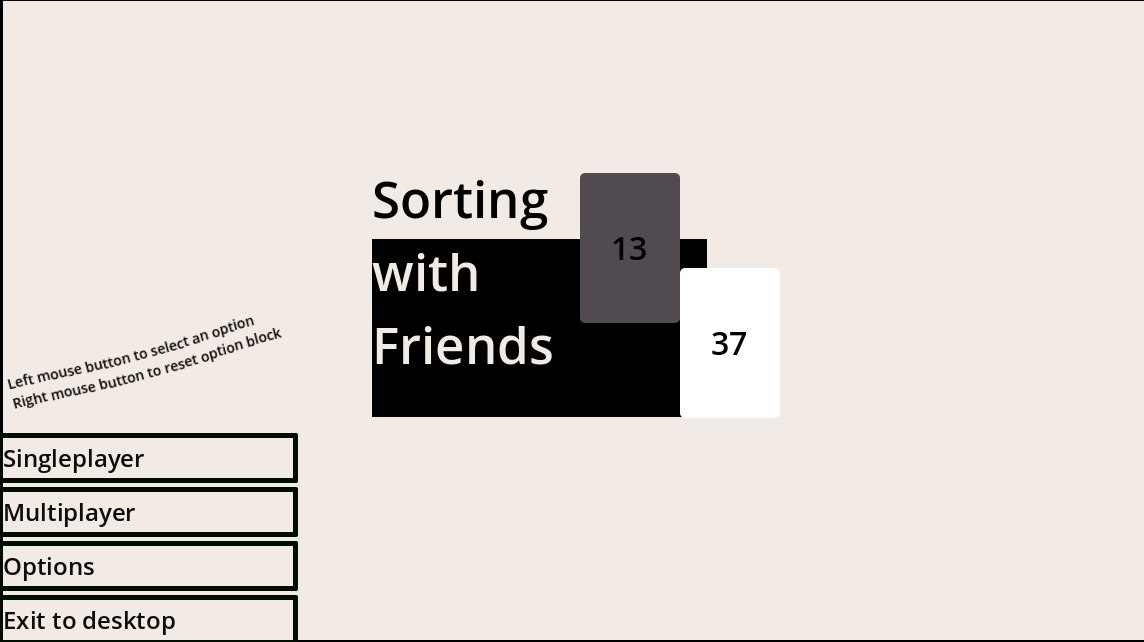
\includegraphics[width=\textwidth]{resources/images/main-menu/main-menu-scene.png}
        \caption{Main menu}
    \end{subfigure}
    \hfill
    \begin{subfigure}[b]{0.45\textwidth}
        \centering
        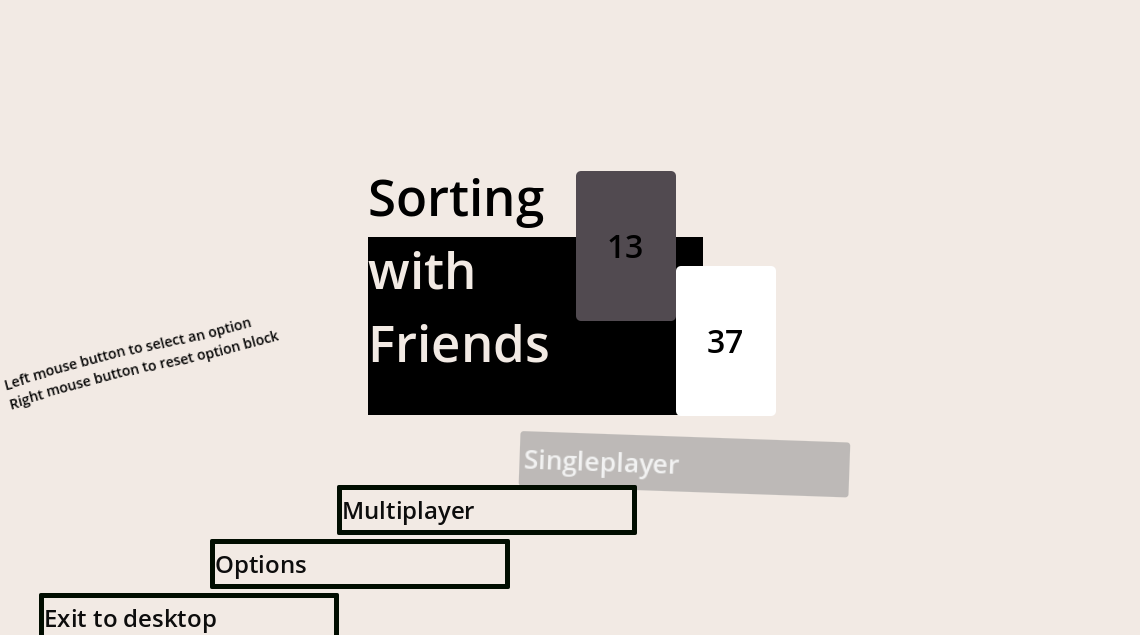
\includegraphics[width=\textwidth]{resources/images/main-menu/main-menu-scene-moving.png}
        \caption{Evasive menu interaction}
    \end{subfigure}
    \caption{Main menu screenshots, including the playful evasive rotating menu microinteraction}
    \label{fig:results-main-menu}
\end{figure}


\begin{figure}[htbp]
    \centering
    \begin{subfigure}[b]{0.45\textwidth}
        \centering
        % TODO This images should be a separated images
        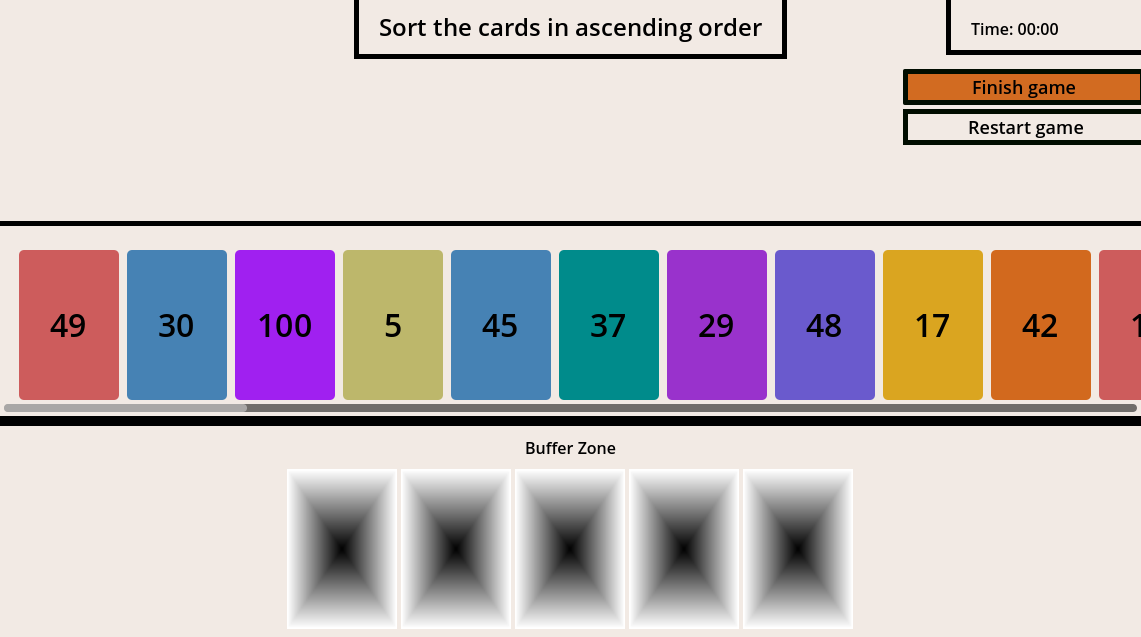
\includegraphics[width=\textwidth]{resources/images/singleplayer/single-player-game.png}
        \caption{Single-player board}
    \end{subfigure}
    \hfill
    \begin{subfigure}[b]{0.45\textwidth}
        \centering
        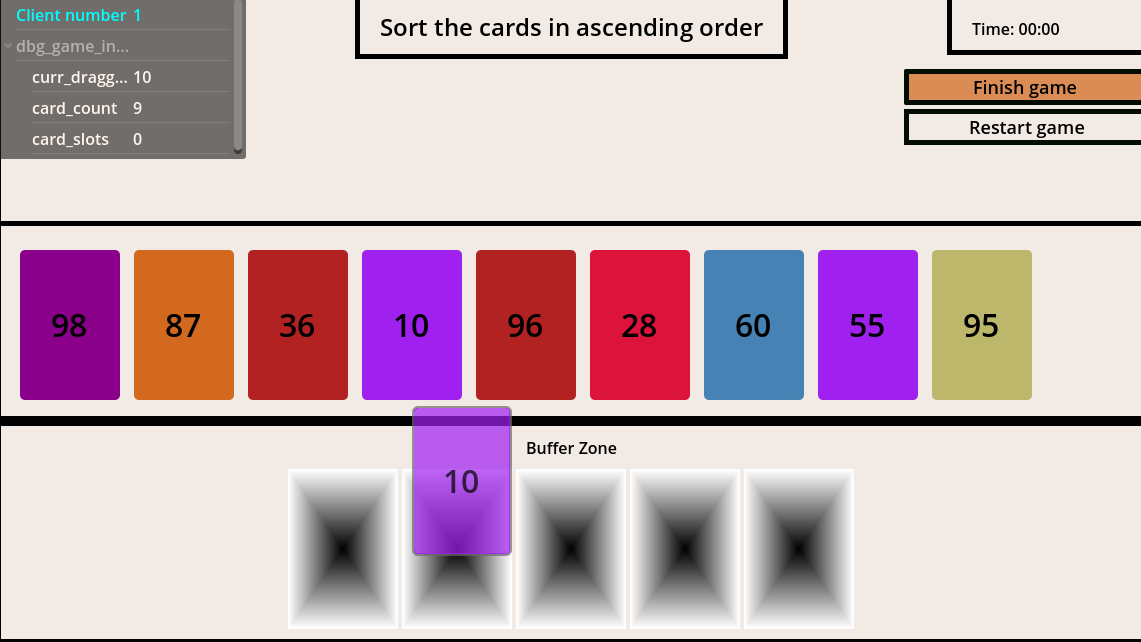
\includegraphics[width=\textwidth]{resources/images/singleplayer/single-player-moving-card.png}
        \caption{Card drag interaction}
    \end{subfigure}
    \caption{Single-player gameplay: board overview and card drag interaction}
    \label{fig:results-singleplayer-gameplay}
\end{figure}

\begin{figure}[htbp]
    \centering
    \begin{subfigure}[b]{0.45\textwidth}
        \centering
        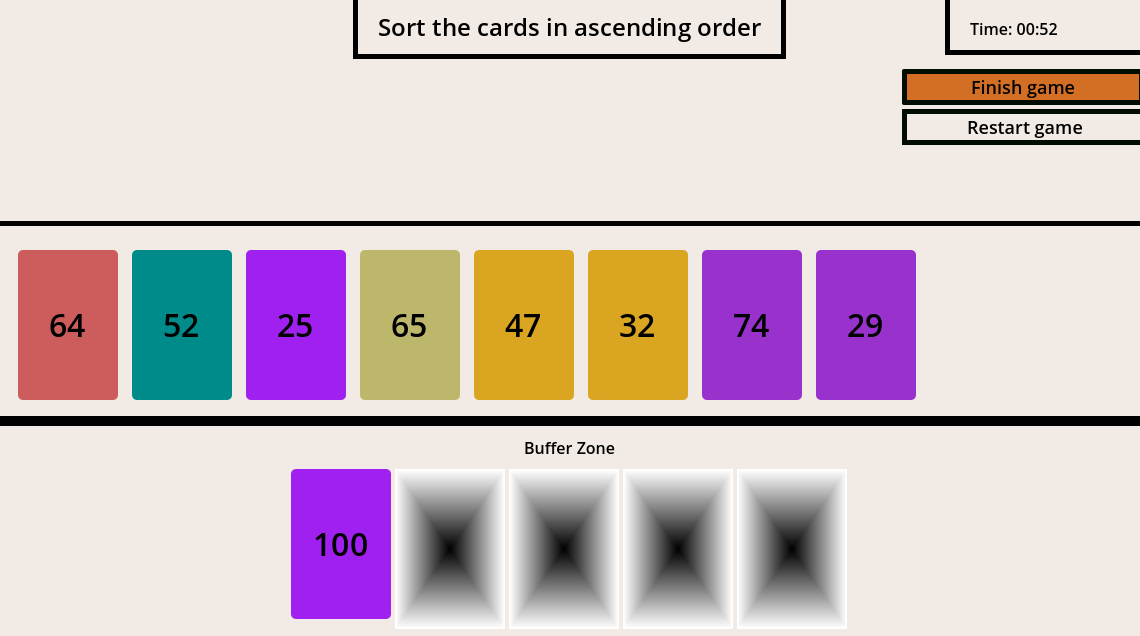
\includegraphics[width=\textwidth]{resources/images/singleplayer/single-player-buffer-card-01.png}
        \caption{Player buffer interaction}
    \end{subfigure}
    \hfill
    \begin{subfigure}[b]{0.45\textwidth}
        \centering
        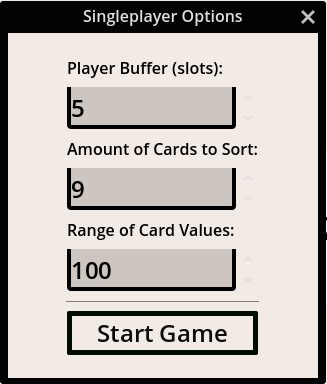
\includegraphics[width=\textwidth]{resources/images/singleplayer/single-player-options.png}
        \caption{Gameplay options}
    \end{subfigure}
    \caption{Player buffer zone usage and in-game options panel}
    \label{fig:results-buffer-options}
\end{figure}

\begin{figure}[htbp]
    \centering
    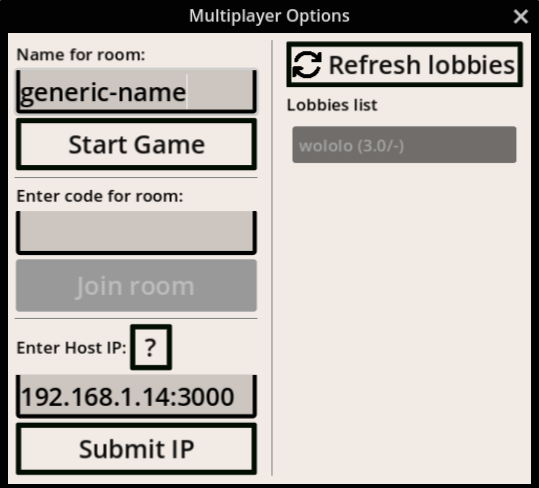
\includegraphics[width=0.62\textwidth]{resources/images/multiplayer/multiplayer-options.png}
    \caption{Multiplayer options before lobby entry: submit signaling-server IP, refresh available lobbies, join a selected lobby, or start a game session as host.}
    \label{fig:results-multiplayer-options}
\end{figure}

\begin{figure}[htbp]
    \centering
    % TODO: Export and add victory screen screenshot
    \begin{subfigure}[b]{0.45\textwidth}
        \centering
        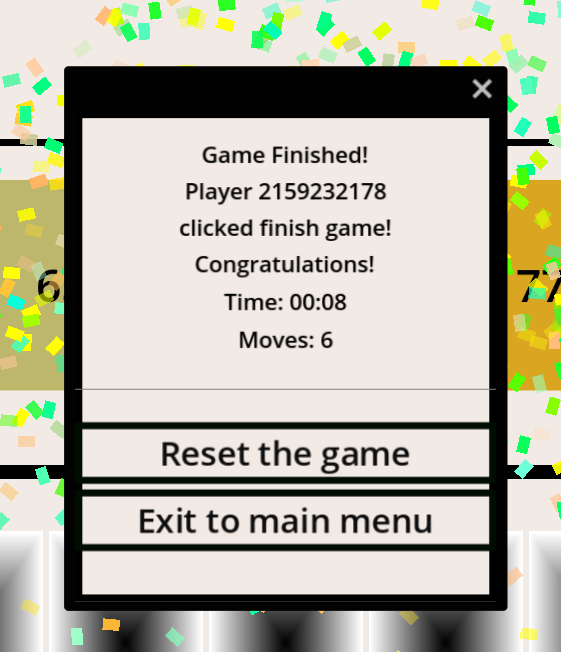
\includegraphics[width=\textwidth]{resources/images/multiplayer/multiplayer-victory.png}
        \caption{Victory screen}
    \end{subfigure}
    \hfill
    \begin{subfigure}[b]{0.45\textwidth}
        \centering
        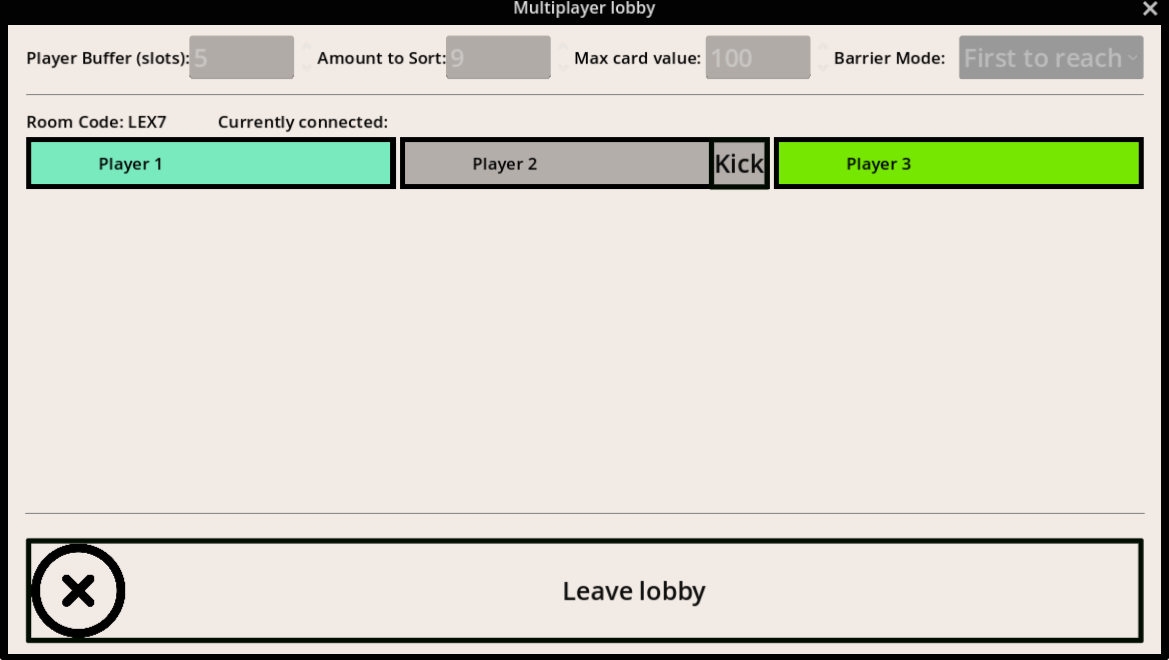
\includegraphics[width=\textwidth]{resources/images/multiplayer/multiplayer-lobby.png}
        \caption{Multiplayer lobby with host and local-player highlighting}
    \end{subfigure}
    \caption{Victory summary and multiplayer lobby with color-coded player identification}
    \label{fig:results-victory-lobby}
\end{figure}

%-----------------------------------------------------------------------
\subsection{Educational Features}
\label{subsec:educational-features}

The tool implements pedagogical mappings to HPC concepts:

\begin{table}[htbp]
    \centering
    \caption{Implemented pedagogical features}
    \label{tab:implemented-pedagogical}
    \begin{tabular}{@{}lll@{}}
        \toprule
        \textbf{HPC Concept}     & \textbf{Game Representation} & \textbf{Status}   \\
        \midrule
        Sequential Execution     & Single player mode           & Implemented       \\
        Shared Memory (OpenMP)   & Shared card container        & Implemented       \\
        Per-Thread Work Area     & local buffer zones           & Implemented       \\
        Parallel Execution       & Multiple players working     & Implemented       \\
        Memory Access Overhead   & Network latency              & Implicit          \\
        Speedup                  & Completion time comparison   & Implemented       \\
        Scalability              & Variable card/player counts  & Implemented       \\
        Load Balancing           & Equal card distribution      & Implemented       \\
        Synchronization Barriers & Turn-based phases            & Implemented       \\
        Race Conditions          & Concurrent card access       & Observable effect \\
        \bottomrule
    \end{tabular}
\end{table}

%-----------------------------------------------------------------------

%-----------------------------------------------------------------------
\subsection{Representative Use Cases}
\label{subsec:use-cases}

The following use cases summarize how the tool was used and what was observed in practice.

\paragraph*{Use Case 1: Instructor-Guided Introductory Session}
\begin{itemize}
    \item \textbf{Context}: Short classroom introduction before formal OpenMP lecture.
    \item \textbf{Activity}: Students first complete a single-player round, then collaborate in multiplayer.
    \item \textbf{Observed behavior}: Participants quickly identified the difference between individual and shared work organization.
    \item \textbf{Outcome}: Faster conceptual entry into shared-memory discussion and more concrete questions during debrief.
\end{itemize}

\paragraph*{Use Case 2: First-Time Multiplayer Coordination}
\begin{itemize}
    \item \textbf{Context}: Small groups (2--10 players) with minimal upfront instructions.
    \item \textbf{Activity}: Player negotiate before starting who handles which card ranges then proceed to sort card collaboratively.
    \item \textbf{Observed behavior}: Na\"{i}ve strategies (e.g.\ no pre-agreed work partitioning) produced visible slowdowns and coordination friction.
    \item \textbf{Outcome}: Users recognized that parallel activity alone is insufficient without coordination discipline.
\end{itemize}

\paragraph*{Use Case 3: Comparative Reflection Session}
\begin{itemize}
    \item \textbf{Context}: Post-game discussion using timer/move outcomes and observed interaction patterns.
    \item \textbf{Activity}: Teams compare sequential baseline and multiplayer performance, then discuss bottlenecks.
    \item \textbf{Observed behavior}: Students linked delays and contention to communication/synchronization overhead.
    \item \textbf{Outcome}: Improved articulation of trade-offs between speedup potential and coordination cost.
\end{itemize}

%-----------------------------------------------------------------------
\subsection{Expected Messages Learned by Users}
\label{subsec:learner-messages}

Based on observed sessions and questionnaire/interview outcomes, the tool is expected to communicate the following messages:

\begin{enumerate}
    \item \textbf{Parallel work can improve completion time, but coordination overhead is real.}
          Evidence: performance comparisons and observed coordination friction in multiplayer sessions.

    \item \textbf{Shared and private workspaces have different roles.}
          Evidence: players recognized shared container access versus local buffer semantics in multiplayer mode.

    \item \textbf{Work balancing strongly affects team performance.}
          Evidence: uneven task distribution corresponded to slower completion and higher perceived confusion.

    \item \textbf{Visibility/synchronization rules shape collaboration behavior.}
          Evidence: hidden public-buffer state and authoritative synchronization influenced player strategy and timing.
\end{enumerate}

These messages align with the architecture/implementation choices documented in Chapters~\ref{ch:architecture} and~\ref{ch:implementation}, and with limitations discussed in Chapter~\ref{ch:problems}.

%-----------------------------------------------------------------------
\subsection{Engagement Effects}
\label{subsec:engagement-effects}

Early usability sessions indicated that small non-critical interaction details affected perceived engagement. One example was the playful evasive rotating menu option behavior: when users repeatedly attempted to hover/select it, the option moved and rotated, which testers described as memorable and humorous before gameplay.

% TODO: [Artifact] Engagement evidence snippet (quote summary or categorized feedback count).
% TODO: [Purpose] Support the claim that microinteractions positively influenced first-impression engagement.
% TODO: [Source Inputs] Early tester notes/interview comments and simple count of positive vs neutral reactions.
% TODO: [Placement] End of this subsection.
% TODO: [Done Criteria] Include at least one summarized quote category and one small count-based indicator.
% TODO: [Cross-refs] Chapter~\ref{ch:architecture}, Section~\ref{sec:responsive-ui-ux}; Section~\ref{subsec:usability-findings}.

\section{Technical Performance}
\label{sec:technical-performance}

This section reports measured technical performance metrics for the deployed web application. Because the game uses an event-driven architecture with no per-frame game logic (\texttt{\_process()} is not used), traditional frame rate benchmarks are not meaningful---the engine's idle render loop runs at the display's native refresh rate regardless of game complexity. Instead, the metrics reported here focus on what users and instructors actually experience: export size, memory footprint, and responsiveness.

%-----------------------------------------------------------------------
\subsection{Load Time and Responsiveness}
\label{subsec:load-time}

The uncompressed \exportSizeUncompressed~MB export loads in under 2~seconds on localhost; real-world load times depend on hosting infrastructure and user bandwidth. Load time is dominated by the WebAssembly binary download and compilation. Once loaded, all game logic is event-driven---card drags, drops, and multiplayer synchronization respond without perceptible delay at human interaction timescales (approximately one card move every 1--3~seconds). The HTTP/SSE relay architecture (Section~\ref{subsec:http-sse-selection}) adds one network hop compared to peer-to-peer, but this overhead remains imperceptible for a turn-based card-sorting game.

%-----------------------------------------------------------------------
\subsection{Memory Usage}
\label{subsec:memory}

Memory consumption was measured using Chrome Task Manager (\texttt{Shift+Esc}) during gameplay sessions across all game states: main menu, single-player with 50, 100, and 200 cards, multiplayer lobby, and multiplayer game.

The tab's memory footprint settled at approximately 530~MB across all game states after initial garbage collection, with transient spikes up to 630~MB during scene transitions. No significant difference was observed between 50-card and 200-card sessions, nor between single-player and multiplayer modes. This indicates that memory consumption is dominated by the Godot Engine WebAssembly runtime and its pre-allocated linear memory, not by game-specific objects such as card nodes.

\paragraph*{Analysis:}

\begin{itemize}
    \item The $\sim$530~MB baseline is well within modern browser limits (typically several GB available per tab) and suitable for classroom computers
    \item Increasing card count from 50 to 200 does not measurably increase memory, confirming that UI nodes are lightweight relative to the engine baseline
    \item No memory leaks were observed---values remained stable after settling, with fluctuations attributable to browser garbage collection cycles
\end{itemize}

%-----------------------------------------------------------------------
\subsection{Web Export Size}
\label{subsec:export-size}

The final web export package characteristics:

\begin{itemize}
    \item \textbf{Uncompressed}: \exportSizeUncompressed~MB
    \item \textbf{Gzip compressed}: \exportSizeGzip~MB
\end{itemize}

\paragraph*{Size Breakdown:}

Godot's web export produces a small number of files rather than a traditional asset tree. The WebAssembly runtime is split across two files, while all game content (scenes, scripts, textures, fonts, and addon code including GDSync) is bundled into a single \texttt{.pck} archive:

\begin{table}[htbp]
    \centering
    \caption{Web export file sizes}
    \label{tab:export-size-breakdown}
    \begin{tabular}{@{}llr@{}}
        \toprule
        \textbf{File}            & \textbf{Contents}                 & \textbf{Size (MB)}               \\
        \midrule
        \texttt{index.pck}       & Scenes, scripts, assets, GDSync   & 90.4                             \\
        \texttt{index.side.wasm} & Godot Engine WASM (main)          & 38.9                             \\
        \texttt{index.js}        & JavaScript glue code              & 2.8                              \\
        \texttt{index.wasm}      & Godot Engine WASM (secondary)     & 1.5                              \\
        \texttt{index.html}      & Entry page                        & 0.01                             \\
        Other                    & Icons, worklets                   & 1.9                              \\
        \midrule
        \textbf{Total}           &                                   & \textbf{\exportSizeUncompressed} \\
        \textbf{Gzip total}      & \textit{(at compression level 6)} & \textbf{\exportSizeGzip}         \\
        \bottomrule
    \end{tabular}
\end{table}

\paragraph*{Comparison:}

The uncompressed export totals \exportSizeUncompressed~MB, reducing to \exportSizeGzip~MB with gzip compression (level~6). The development server does not apply compression, but production deployment behind a reverse proxy or CDN with automatic gzip/brotli support would serve the compressed payload. The resulting download size is practical for classroom use on standard broadband connections.

\paragraph*{Note on the development server:}

The Python-based HTTPS server used for LAN testing (\texttt{exports/main.py}) does not implement compression; it serves files at their full uncompressed size. This is acceptable for LAN testing where bandwidth exceeds 100~Mbps, but production deployment should use a server or CDN that supports \texttt{Content-Encoding: gzip}.

%-----------------------------------------------------------------------
\section{Platform Compatibility}
\label{sec:platform-compatibility}

%-----------------------------------------------------------------------
\subsection{Browser Compatibility}
\label{subsec:browser-compatibility}

Testing conducted across major web browsers:

\begin{table}[htbp]
    \centering
    \caption{Browser compatibility}
    \label{tab:browser-compat}
    \begin{tabular}{@{}lccl@{}}
        \toprule
        \textbf{Browser} & \textbf{Platform} & \textbf{Status} & \textbf{Notes}             \\
        \midrule
        Chrome 145+      & Windows           & Functional      & Reference browser          \\
        Firefox 148+     & Windows           & Functional      & Independent engine (Gecko) \\
        Edge 145+        & Windows           & Functional      & Chromium-based             \\
        \bottomrule
    \end{tabular}
\end{table}

\paragraph*{Minimum Requirements:}

\begin{itemize}
    \item Modern browser with WebGL 2.0 and WebAssembly support
    \item 2 GB available RAM recommended
    \item Internet connection for multiplayer
    \item JavaScript enabled
\end{itemize}

%-----------------------------------------------------------------------
\subsection{Responsive Layout}
\label{subsec:responsive-layout}

The game adapts to various screen configurations:

\begin{itemize}
    \item \textbf{Small windows (< 800px width)}: Compact layout with scrollable cards
    \item \textbf{Medium windows (800--1200px)}: Optimal experience, target size range
    \item \textbf{Large windows (> 1200px)}: Excellent, plenty of space for all elements
\end{itemize}

\paragraph*{Input Support:}

\begin{itemize}
    \item \textbf{Mouse}: Full support with click-and-drag interactions
    \item \textbf{Touch}: Supported for touchscreen displays and tablets
    \item Responsive layout adjustment on window resize
\end{itemize}

%-----------------------------------------------------------------------
% \section{Usability Evaluation}
% \label{sec:usability-evaluation}
% % TODO: [Artifact] Usability visualization set (Likert summary + feedback category breakdown).
% % TODO: [Purpose] Make qualitative/quantitative usability outcomes scannable and auditable.
% % TODO: [Source Inputs] Questionnaire items in Section~\ref{subsec:informal-testing}; positive/improvement findings in Section~\ref{subsec:usability-findings}.
% % TODO: [Placement] At the beginning of this section.
% % TODO: [Done Criteria] Provide one aggregated Likert chart and one categorized feedback chart with participant counts matching reported text.
% % TODO: [Cross-refs] Section~\ref{subsec:engagement-effects}; Chapter~\ref{ch:problems}, Section~\ref{sec:mobile-ux-challenges}.


%-----------------------------------------------------------------------
\section{Educational Effectiveness}
\label{sec:educational-effectiveness}

%-----------------------------------------------------------------------
\subsection{Preliminary Assessment}
\label{subsec:preliminary-assessment}

While formal educational efficacy evaluation is outside the scope of this thesis, preliminary indicators suggest the following educational value:

\paragraph*{Quantitative HPC Metrics:}

To evaluate educational effectiveness, HPC performance concepts can be introduced during gameplay:

\begin{itemize}
    \item \textbf{Speedup ($S$)}: Defined as $S = T_1 / T_p$ where $T_1$ is single-player completion time and $T_p$ is $p$-player completion time.
    \item \textbf{Efficiency ($E$)}: Calculated as $E = S / p = T_1 / (p \cdot T_p)$.
    \item \textbf{Communication Overhead}: Time spent passing cards between players (analogous to message passing cost in distributed systems).
    \item \textbf{Load Imbalance}: Observable when one player receives more difficult cards or falls behind, reducing overall parallel efficiency.
\end{itemize}



%-----------------------------------------------------------------------
\subsection{Pedagogical Value Proposition}
\label{subsec:pedagogical-value}

The game serves as an effective \textbf{icebreaker or introductory activity}:

\begin{itemize}
    \item \textbf{Pre-Lecture Activity}: Introduce concepts before formal instruction
    \item \textbf{Discussion Starter}: Generate questions and curiosity about parallel computing
    \item \textbf{Concept Visualization}: Provide mental model for abstract concepts
    \item \textbf{Reinforcement Tool}: Practice and reinforce learned concepts
    \item \textbf{Assessment Aid}: Reveal misconceptions for instructors to address
\end{itemize}

%-----------------------------------------------------------------------
\subsection{Comparison with Traditional Methods}
\label{subsec:comparison-traditional}

Informal comparison with traditional HPC teaching methods:

\begin{table}[htbp]
    \centering
    \caption{Expected advantages over traditional methods}
    \label{tab:comparison-traditional}
    \begin{tabular}{@{}lcc@{}}
        \toprule
        \textbf{Criterion}          & \textbf{Game} & \textbf{Lecture/Textbook} \\
        \midrule
        Engagement                  & High          & Medium-Low                \\
        Immediate Feedback          & Yes           & No                        \\
        Hands-On Experience         & Yes           & No                        \\
        Conceptual Visualization    & Strong        & Weak                      \\
        Detailed Explanation        & Weak          & Strong                    \\
        Accessibility               & High          & Medium                    \\
        Scalability (student count) & High          & Medium                    \\
        \bottomrule
    \end{tabular}
\end{table}

\paragraph*{Conclusion:}

The tool is not a replacement for traditional instruction, but a complementary, instructor-guided activity that can enhance engagement and provide intuitive understanding before formal study.

%-----------------------------------------------------------------------
\section{Comparison with Initial Requirements}
\label{sec:requirements-comparison}

%-----------------------------------------------------------------------
\subsection{Requirements Fulfillment}
\label{subsec:requirements-fulfillment}

Assessment of how well the completed system meets the requirements defined in Section~\ref{sec:requirements}:

\begin{table}[htbp]
    \centering
    \caption{Requirements fulfillment status}
    \label{tab:requirements-status}
    \begin{tabular}{@{}llc@{}}
        \toprule
        \textbf{Category} & \textbf{Requirement}             & \textbf{Status} \\
        \midrule
        Functional        & FR1: Card management             & \checkmark Met  \\
                          & FR2: Single-player mode          & \checkmark Met  \\
                          & FR3: Multiplayer mode            & \checkmark Met  \\
                          & FR4: User interface              & \checkmark Met  \\
                          & FR5: Feedback \& instrumentation & \checkmark Met  \\
                          & FR6: Configurable difficulty     & \checkmark Met  \\
                          & FR7: Guest access                & \checkmark Met  \\
        \midrule
        Non-Functional    & NFR1: Usability                  & \checkmark Met  \\
                          & NFR2: Reliability                & \checkmark Met  \\
                          & NFR3: Maintainability            & \checkmark Met  \\
        \midrule
        Constraint        & C1: Licensing \& distribution    & \checkmark Met  \\
        \bottomrule
    \end{tabular}
\end{table}

\paragraph*{Notes:}

\begin{itemize}
    \item \textbf{Conceptual Clarity}: Strong for HPC-experienced users; needs educational overlay for beginners

    \item \textbf{Browser Support}: Modern browsers fully supported across platforms
\end{itemize}

%-----------------------------------------------------------------------
\section{Known Limitations}
\label{sec:limitations}

%-----------------------------------------------------------------------
\subsection{Current Limitations}
\label{subsec:current-limitations}

\begin{enumerate}
    \item \textbf{Platform Support}: Currently web-only; native mobile apps not implemented

    \item \textbf{Educational Scaffolding}: Limited in-game explanations; requires instructor context

    \item \textbf{Sorting Algorithm Guidance}: The tool supports static partitioning strategies such as parallel merge sort (see Chapter~\ref{ch:architecture}, Section~\ref{sec:algorithm-mode-extensibility}), but does not support recursive strategies such as parallel quicksort and does not yet provide guided step-by-step modes for specific algorithms

    \item \textbf{Performance Metrics}: Basic timing and moves; lacks detailed profiling (speedup curves, scalability graphs)

    \item \textbf{Advanced HPC Concepts}: Doesn't cover race conditions, deadlocks, synchronization primitives explicitly

    \item \textbf{Automated Assessment}: No built-in assessment or progress tracking for educational use

    \item \textbf{Formal Evaluation}: Lacks comprehensive educational efficacy study
\end{enumerate}

%-----------------------------------------------------------------------
\subsection{Scope Limitations}
\label{subsec:scope-limitations}

Certain features were intentionally deferred to maintain project scope:

\begin{itemize}
    \item User accounts and progress persistence
    \item Leaderboards and social features
    \item Advanced sorting algorithm demonstrations
    \item GPU parallelism (CUDA/OpenCL) simulations
    \item Instructor dashboard for classroom management
    \item Detailed analytics and learning analytics integration
\end{itemize}

%-----------------------------------------------------------------------
\section{Summary}
\label{sec:results-summary}

This chapter presented comprehensive evaluation results:

\begin{itemize}
    \item \textbf{Completed Features}: All core functional and educational features successfully implemented
    \item \textbf{Technical Performance}: Meets or exceeds performance targets on representative devices
    \item \textbf{Platform Compatibility}: Excellent browser compatibility across platforms
    \item \textbf{Usability}: Generally positive usability feedback with actionable improvement suggestions
    \item \textbf{Educational Effectiveness}: Preliminary evidence suggests value as introductory/supplementary tool
    \item \textbf{Requirements Fulfillment}: Nearly all initial requirements met or exceeded
    \item \textbf{Limitations}: Known limitations documented for transparency and future work planning
\end{itemize}

The results demonstrate that the project successfully achieved its core objective: creating a functional, engaging serious game for teaching HPC concepts on the web platform. The next chapter evaluates the completed system and presents performance metrics and assessment results.